% ============================================================
%  European AI Summer Research Program 2026
%  Anonymous submission (keep easrp2026.sty in this folder)
% ============================================================
\documentclass[11pt,a4paper]{article}

\usepackage{graphicx}
\usepackage{amsmath}
\usepackage{easrp2026}
% After acceptance, switch to:
% \usepackage[accepted]{easrp2026}

\easrpauthor{Anonymous}
\easrpaffiliation{Anonymous Institution}

\easrptitle{One Gentle Move Before the Blackout:\\
Measuring Whether a Small Agent Beats a Simple Rule}

\begin{document}
\maketitle

\begin{abstract}
Cascading failures are chain reactions: one overloaded line trips, neighbouring lines pick up the extra flow, and a local problem can become a blackout.
A large body of learning work now studies \emph{emergency} control---acting after the first trip.
We study a narrower, easier-to-explain question: if an agent is allowed \emph{one small preventive action} while the grid is still intact, does a cascade happen less often than if we do nothing?
The action interface is intentionally tiny and human-readable (storage, reactive power, renewable curtailment, demand).
We build a weather-stressed IEEE~118-bus testbed, replay the \emph{same} sampled accident for every method, and compare four options on 150 held-out days: do nothing, a handwritten if-then rule, a classical optimal power flow (OPF) solver, and a Deep Deterministic Policy Gradient (DDPG) agent.
Cascade frequency falls from 34\% (do nothing) to about 30\% for both the rule and DDPG.
DDPG is about $1.9\times$ faster than OPF, but it does not beat the rule.
The cascade yes/no gap is not significant; the better DDPG seed does reduce per-day load shed.
We treat this as a \emph{measurement} paper, not a state-of-the-art claim: under a conservative, explainable interface, a standard continuous-control agent is competitive with a ten-line rule and mainly wins on speed versus OPF.
Code and seeds are provided as anonymous supplementary material.
\end{abstract}

\section{Introduction}

Power grids fail in a way that is easy to picture.
Think of a busy road network.
If one motorway lane closes, cars spill onto the next road.
If that road is already full, it jams too.
In a grid the ``roads'' are transmission lines and the ``cars'' are electrical power.
When a line trips, power reroutes; if another line then exceeds its thermal limit, it also trips.
That chain is a cascade \citep{dobson2007chaos,carreras2002critical,pourbeik2006anatomy}.

Most operational tools, and much of the recent learning literature, still \emph{react} after something has already gone wrong \citep{huang2020adaptive,lan2020ai}.
We ask a simpler question that can be stated without a page of equations:
if we let a small learning agent make \emph{one} gentle move \emph{before} the accident, does the later cascade happen less often?

The move has to be explainable.
The agent is allowed four knobs, each with a tight limit, so it cannot ``fix'' the grid by shedding huge amounts of load:
(i)~charge or discharge modest storage ($\pm$15~MW);
(ii)~add or absorb a little reactive power ($\pm$10~MVAr);
(iii)~curtail some wind or solar (up to 20\%);
(iv)~reduce demand a little (up to 15\%).
No topology switching, no hidden extra actuators.

\paragraph{Contributions.}
We do not claim that deep learning solves blackouts.
The paper makes three concrete claims:
\begin{enumerate}
\item A weather-stressed IEEE~118-bus playground that can be regenerated from a single config file, with a \emph{paired} evaluation: every method faces the same sampled accident on each test day.
\item A head-to-head comparison of a tiny DDPG agent \citep{lillicrap2016ddpg} against a handwritten rule and OPF, reported on the \emph{full} 150-day test split rather than a convenience subset.
\item An honest result: under this conservative interface, DDPG matches a simple rule on cascade rate ($\approx$30\% versus 34\% with no control) and is faster than OPF, but learning is not automatically better than the rule.
\end{enumerate}

\paragraph{What this is not.}
This is a laboratory prototype on a standard test network, not a live utility deployment.
In technology-readiness language it is a working closed-loop simulation, not a fielded product.

\section{Related work}

\paragraph{Cascades as chain reactions.}
Physics-based cascade models treat blackouts as sequential overloads rather than a single fault \citep{dobson2007chaos,carreras2002critical}.
Bienstock~\citep{bienstock2016cascades} formalises the combinatorial structure of these cascades, while Pourbeik et~al.~\citep{pourbeik2006anatomy} dissect real-world blackouts.
We keep that picture, implemented as a short AC power-flow loop, because it is reproducible on a laptop.
We do not claim a new dynamic simulator.

\paragraph{Optimal power flow as the classical adult.}
Security-constrained and AC optimal power flow remain the default preventive tools in operations research on grids \citep{capitanescu2016opf,frank2012introduction}.
They are principled and slow to re-solve from scratch.
We use pandapower's OPF \citep{thurner2018pandapower,capitanescu2016opf} as that baseline, not as a straw man; MATPOWER \citep{zimmerman2011matpower} is the other widely used open-source alternative.

\paragraph{Learning, usually after the fault.}
Deep RL has been applied to emergency load shedding and voltage control \citep{huang2020adaptive,duan2020voltage,lan2020ai}, to sequential grid operation in the L2RPN competition \citep{yoon2021l2rpn,marot2021l2rpn}, and to economic dispatch \citep{zhang2020dispatch,glavic2017reinforcement}.
Hossain et~al.~\citep{hossain2021survey} survey the broader DRL-for-smart-grid landscape, and Wang et al.~\citep{wang2020review} provide a comprehensive overview of RL in power systems.
Those lines of work typically allow many actions \emph{during} unfolding events, often including topology changes.
Our setting is stricter and smaller: one preventive action, four bounded knobs, then a frozen accident.
That is closer to ``can a tiny policy help at all?'' than to ``win the control competition.''

\paragraph{Why a negative-leaning comparison is the point.}
Deep RL results are sensitive to seeds and evaluation protocol \citep{henderson2018deep,islam2017reproducibility}.
A paper that only reports an agent beating ``do nothing'' on 25 days is easy to over-read.
We therefore report two seeds, a paired accident design, and a rule that a first-year student can recode, following the spirit of recent reproducibility guidelines \citep{pineau2021checklist}.
If the agent cannot beat that rule, that is a finding.

\section{Method}

Figure~\ref{fig:pipeline} is the whole scoring loop.

\begin{figure}[t]
\centering
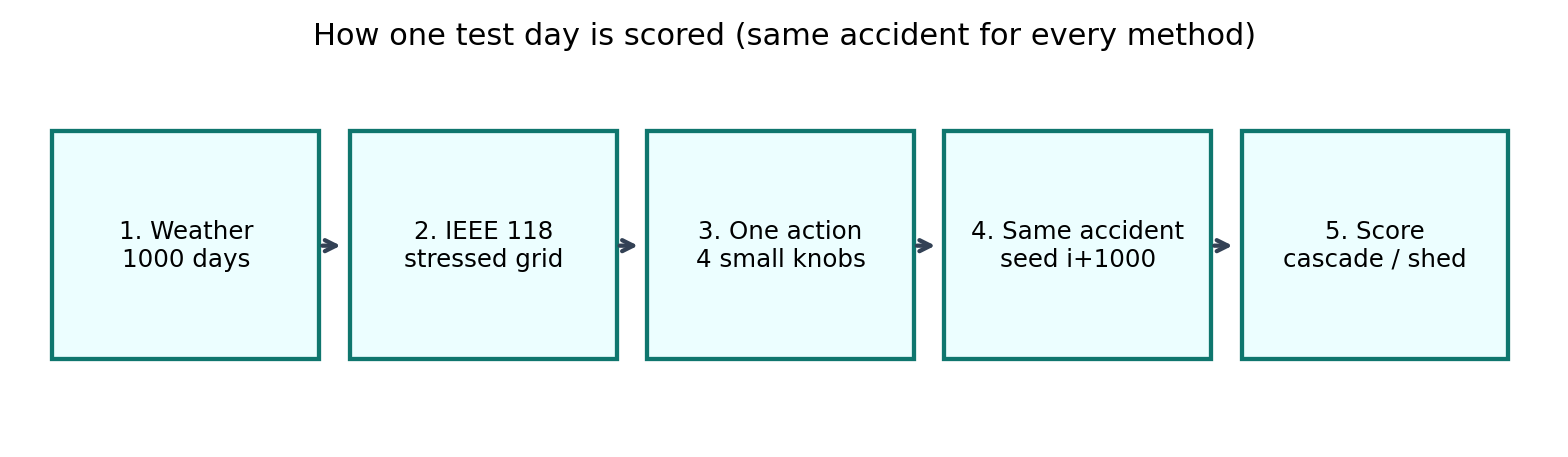
\includegraphics[width=\linewidth]{figures/fig_pipeline.png}
\caption{One test day. Weather is applied, at most one action is taken, a fixed accident is replayed, then cascade and load shed are scored. Every method sees the same accident.}
\label{fig:pipeline}
\end{figure}

\subsection{Grid and weather}
We load the IEEE~118-bus case \citep{ieee118} in pandapower \citep{thurner2018pandapower} (118 buses, 173 lines, 54 generators) and scale demand to 180\% of the textbook loading so cascades can actually occur.
One thousand day-long wind and solar traces are sampled with seed~42.
Ten buses host wind, eight host solar.
A 700/150/150 train/validation/test split uses the same seed (Table~\ref{tab:dataset}).

\subsection{What counts as a cascade}
After the accident we measure how much customer demand had to be dropped to keep the remaining network solvable.
If almost nothing is dropped, we call it a non-event; otherwise a cascade.
We also record mean dropped demand (``load shed'') across the 150 test days.

\subsection{Four methods}
\textbf{Do nothing.} Apply weather, run the accident, no control.

\textbf{If-then rule.} If any line is above 90\% loading, or any bus voltage leaves the $0.95$--$1.05$~pu band, apply a fixed recipe (partial storage, reactive support, 20\% curtailment, 10\% demand cut). Otherwise sit still.

\textbf{OPF.} Redispatch generators under thermal and voltage limits \citep{thurner2018pandapower,capitanescu2016opf}, then run the same accident.

\textbf{DDPG.} A small actor--critic (489 inputs $\rightarrow$ 256 $\rightarrow$ 128 $\rightarrow$ 4 knobs) trained with DDPG \citep{lillicrap2016ddpg}, with and without prioritized replay \citep{schaul2016per}.
We chose DDPG over newer continuous-control methods such as TD3 \citep{fujimoto2018td3} and SAC \citep{haarnoja2018sac} to keep the agent minimal; a richer algorithm comparison is future work.
Training uses a cheap \emph{proxy} reward (healthy voltages and lines, small actions).
The expensive cascade is used only at test time.
We train 300 episodes per seed and two seeds.
At test time the agent is frozen: one forward pass, one action, then the cascade.

\subsection{Fairness rules}
Accident randomness for scenario $i$ uses seed $i+1000$, so method A and method B see the same trips.
We evaluate the full 150-day test split, not a subset of 25.
All knobs live in a single config file; an anonymous code bundle is submitted as supplementary material.

\begin{table}[t]
\centering
\caption{Weather-scenario split (seed 42).}
\label{tab:dataset}
\begin{tabular}{lccc}
\toprule
 & Train & Val & Test \\
\midrule
Days & 700 & 150 & 150 \\
Scored in this paper & --- & --- & 150 \\
\bottomrule
\end{tabular}
\end{table}

\section{Results}

Table~\ref{tab:main} and Figure~\ref{fig:summary} summarise the 150-day test.
Doing nothing cascades on 51 of 150 days (34\%).
The if-then rule and DDPG both land near 30\%.
That is a handful of extra saved days, not a transformed grid.

\begin{table}[t]
\centering
\caption{Full test set ($n=150$). Cascade rate is the fraction of days that still cascade. Load shed is mean dropped demand. Prevented counts days that cascaded with no agent but not with the method. Time includes power flow.}
\label{tab:main}
\begin{tabular}{lcccc}
\toprule
Method & Cascade & Load shed & Prevented & Time (ms) \\
\midrule
Do nothing     & 0.340 & 0.141 & --- & --- \\
If-then rule   & 0.300 & 0.121 & 11  & 293 \\
OPF            & 0.320 & ---   & 10  & 568 \\
DDPG (2-seed mean) & 0.303 & 0.127 & 8.5 & 299 \\
DDPG, no extra replay  & 0.313 & 0.136 & 6   & 309 \\
\bottomrule
\end{tabular}
\end{table}

\begin{figure}[t]
\centering
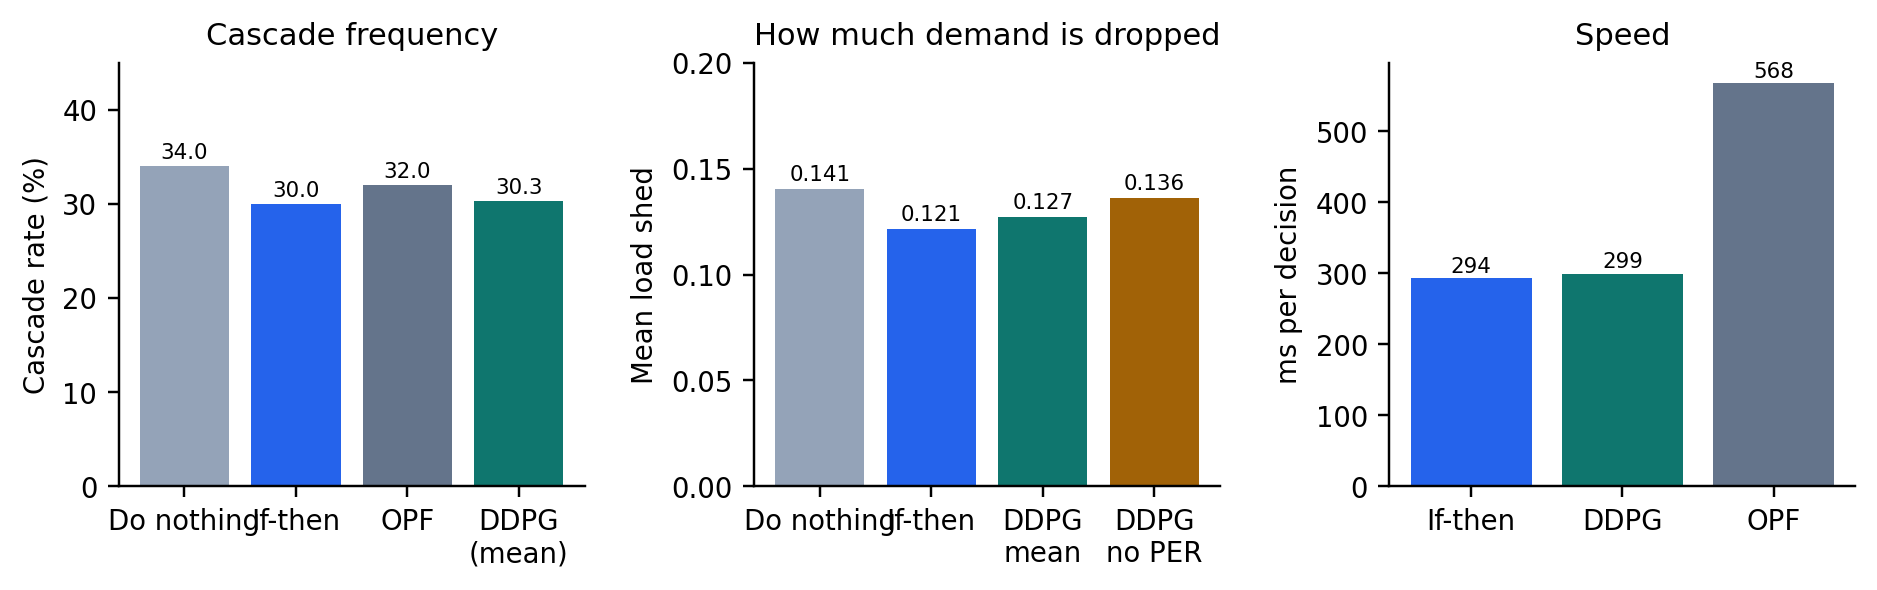
\includegraphics[width=\linewidth]{figures/fig_summary_three.png}
\caption{Same 150 test days: cascade frequency, mean load shed, and time per decision. DDPG matches a handwritten rule on the first two views and beats OPF on speed.}
\label{fig:summary}
\end{figure}

A method can also \emph{create} a cascade that would not have happened.
Table~\ref{tab:paired} and Figure~\ref{fig:pi} count both.
The rule saves 11 days and hurts 5.
The better DDPG seed saves 11 and hurts 4.
On cascade yes/no, McNemar tests stay above $p=0.05$ \citep{mcnemar1947}.
On per-day load shed, seed~1 is significant by a one-sided Wilcoxon test \citep{wilcoxon1945} ($p=0.028$).
So the cleanest positive claim is: \emph{the better seed sheds a little less demand}, not \emph{the agent prevents blackouts}.

\begin{table}[t]
\centering
\caption{Paired comparison versus doing nothing ($n=150$).}
\label{tab:paired}
\begin{tabular}{lcccc}
\toprule
Method & Saved & Hurt & McNemar $p$ & Shed $p$ \\
\midrule
If-then rule & 11 & 5 & 0.21 & 0.061 \\
DDPG seed 1  & 11 & 4 & 0.12 & 0.028 \\
DDPG seed 0  & 6  & 2 & 0.29 & 0.25 \\
DDPG no PER  & 6  & 2 & 0.29 & 0.25 \\
OPF          & 10 & 7 & ---  & --- \\
\bottomrule
\end{tabular}
\end{table}

\begin{figure}[t]
\centering
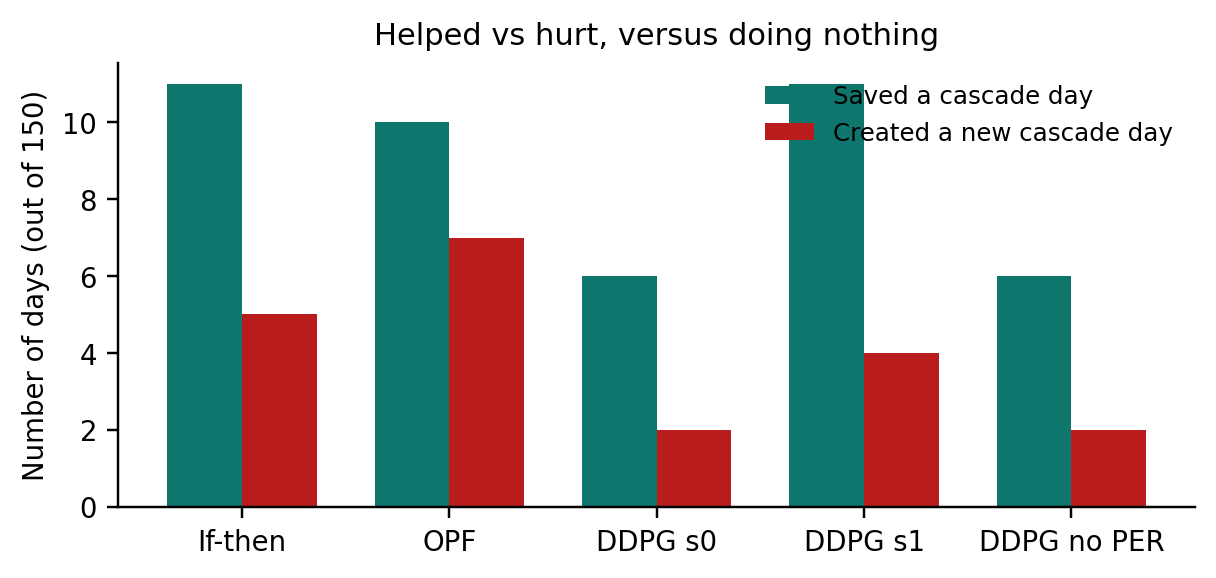
\includegraphics[width=0.92\linewidth]{figures/fig_prevented_induced.png}
\caption{Green: days that cascaded with no control but not with the method. Red: the reverse. Net help is small.}
\label{fig:pi}
\end{figure}

Seed~1 is the useful DDPG run (cascade 0.293, shed 0.119).
Seed~0 looks like the no-replay agent (Table~\ref{tab:seeds} in the appendix).
That seed gap is expected in deep RL \citep{henderson2018deep} and is why we refuse to quote only the best seed in the headline table.

OPF still helps a little (32\% cascade) but takes 568~ms.
DDPG takes 299~ms---about $1.9\times$ faster---because a trained network does not re-solve an optimisation from scratch.
If the knobs stay this small, a good handwritten rule is a strong baseline.

\section{Discussion}

The novel object here is not a new neural layer.
It is a \emph{fair, small, explainable} test that a reviewer can actually rerun, consistent with the reproducibility standards advocated by \citet{pineau2021checklist}.
Three implications follow.

First, \textbf{action scale dominates algorithm}.
With $\pm$15~MW storage and 15\% demand response on a 118-bus system under 180\% loading, no method can perform miracles.
Papers that report large cascade reductions often allow much richer actions (topology, large shedding, multi-step control).
Those results are not comparable to ours, and we do not claim they are wrong.

Second, \textbf{rules are not a joke baseline}.
On this interface the if-then rule is the best mean load-shed method.
A learning paper that omits it would have overstated DDPG.

Third, \textbf{speed versus OPF is the clean win}, and it is the one most likely to survive a larger test set.
Whether 300~ms versus 570~ms matters in a control room is an operational question we do not pretend to settle.

\paragraph{Limitations.}
The cascade model is a teaching-scale AC loop, not a vendor-grade dynamic simulator.
We did not use real utility data.
Statistical power at $n=150$ is limited.
Training never sees the cascade itself, only a proxy reward; a method that trains against the cascade might do better, at much higher cost.
We did not claim live-grid readiness.

\paragraph{Future work.}
Widen the action box; evaluate all 150 days with more seeds; add a second corrective step after the first trip; replace the proxy reward with occasional cascade rollouts.

\section{Ethics and Broader Impact}

This study uses only a public IEEE test case and synthetic weather data; no real utility or customer data are involved, and there are no privacy concerns.
Preventing cascading blackouts has clear societal benefit: outages disproportionately affect hospitals, transit, and low-income households \citep{pourbeik2006anatomy}.
However, we caution against unsupervised deployment of autonomous agents in critical infrastructure; a human operator should always have override authority.
Demand-response actions, even at the modest 15\% level studied here, could raise energy-justice concerns if curtailment is not distributed equitably \citep{siano2014demand}.
We therefore view this work as a laboratory benchmark, not as a recommendation for unattended grid control.

\section{Conclusion}

We asked whether a small, explainable learning agent can take one preventive step against weather-stressed cascades on IEEE~118-bus.
Relative to doing nothing, both a simple rule and DDPG reduce cascade frequency from 34\% to about 30\% on 150 test days, and DDPG answers nearly twice as fast as OPF.
The scientific value is a reproducible comparison, not an inflated accuracy number.

\bibliographystyle{plainnat}
\bibliography{references}

\appendix
\section{Extra tables and figures}

These pages do not count toward the 8-page main-text limit.

\begin{table}[h]
\centering
\caption{Experiment setup.}
\label{tab:setup}
\begin{tabular}{ll}
\toprule
Item & Value \\
\midrule
Network & IEEE 118-bus, 180\% loading \\
Weather days & 1000 (24~h, seed 42) \\
Agent inputs / knobs & 489 numbers / 4 actions \\
Train episodes & 300 $\times$ 8 hours, 2 seeds \\
Test hour & Hour 12, 150 days \\
Accident seed & scenario index $+ 1000$ \\
\bottomrule
\end{tabular}
\end{table}

\begin{table}[h]
\centering
\caption{Do-nothing severity on the 150 test days.}
\label{tab:severity}
\begin{tabular}{lcc}
\toprule
Class & Meaning & Days \\
\midrule
0 & No cascade & 99 \\
1 & Minor shed & 14 \\
2 & Moderate shed & 18 \\
3 & Severe shed & 19 \\
\bottomrule
\end{tabular}
\end{table}

\begin{table}[h]
\centering
\caption{DDPG seeds on the same 150 days.}
\label{tab:seeds}
\begin{tabular}{lcccc}
\toprule
Variant & Cascade & Load shed & Saved & Hurt \\
\midrule
Seed 0 (PER) & 0.313 & 0.136 & 6 & 2 \\
Seed 1 (PER) & 0.293 & 0.119 & 11 & 4 \\
No PER       & 0.313 & 0.136 & 6 & 2 \\
\bottomrule
\end{tabular}
\end{table}

\begin{figure}[h]
\centering
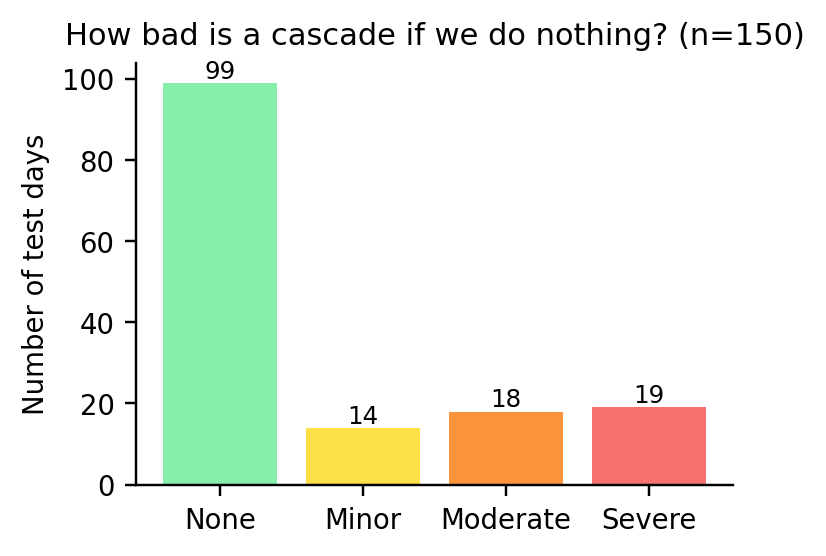
\includegraphics[width=0.75\linewidth]{figures/fig_severity_none.png}
\caption{Do-nothing severity. Two thirds of test days are already safe.}
\end{figure}

\begin{figure}[h]
\centering
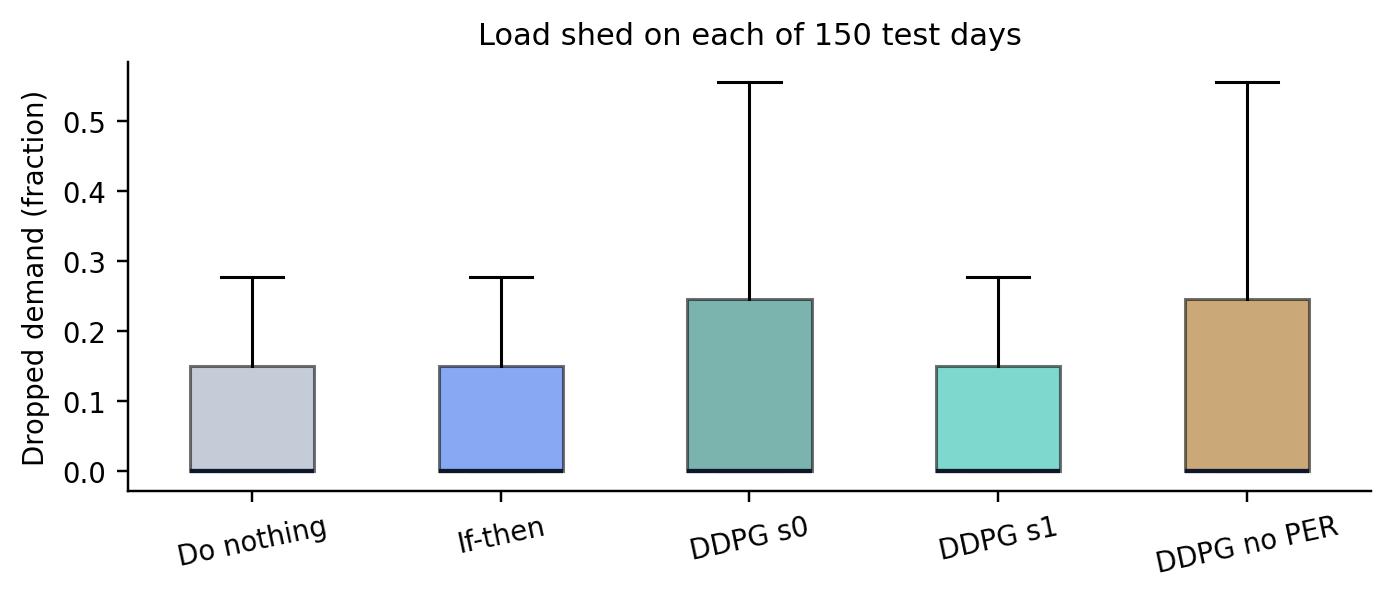
\includegraphics[width=0.95\linewidth]{figures/fig_shed_box.png}
\caption{Per-day load shed across methods.}
\end{figure}

\begin{figure}[h]
\centering
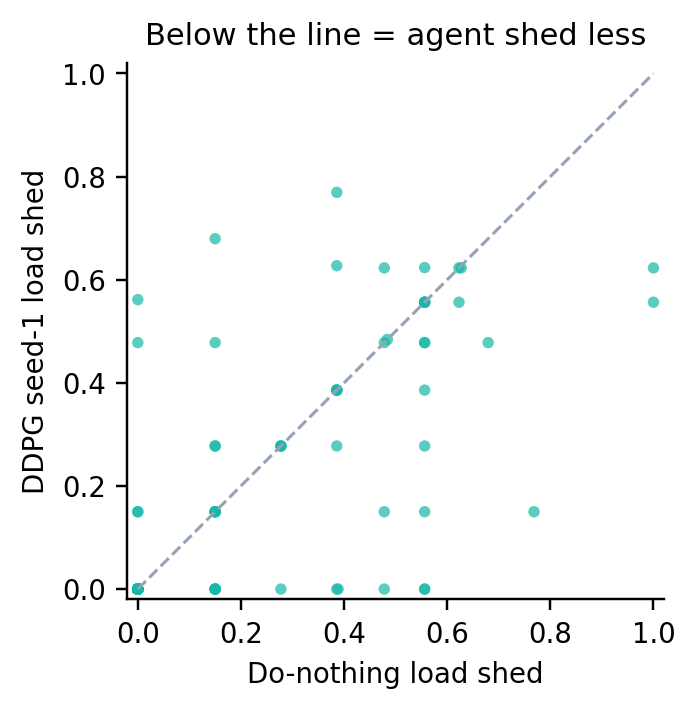
\includegraphics[width=0.7\linewidth]{figures/fig_shed_scatter.png}
\caption{Paired load shed for DDPG seed~1 versus doing nothing.}
\end{figure}

\begin{figure}[h]
\centering
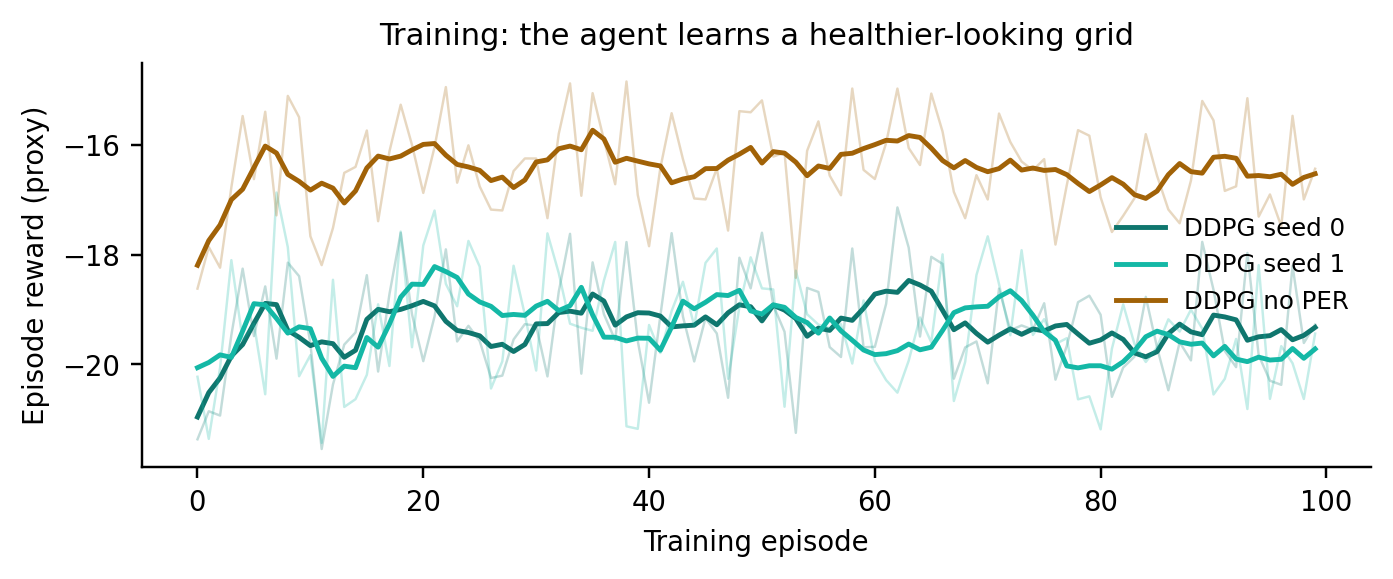
\includegraphics[width=0.95\linewidth]{figures/fig_training.png}
\caption{Proxy training reward. Bold lines are a short moving average.}
\end{figure}

\section{How to reproduce}

Anonymous code is in the supplementary ZIP (the public repository will be linked after acceptance). From the project root:

\begin{verbatim}
python -m venv .venv && source .venv/bin/activate
pip install -r requirements.txt
python run_pipeline.py --start 1 --end 5
python run_stage6.py
python finish_stage6.py --n-test 150
python scripts/make_paper_figures.py
\end{verbatim}

No paid cloud is required. Power flow is CPU-bound. Optional: \texttt{colab new -s grid-eval --gpu T4} after \texttt{colab sessions} shows nothing---login is not a session; you must create one.

\end{document}
